
\documentclass[a4paper,11pt]{article}%,twocolumn
%% packages

\usepackage{blindtext} % needed for creating dummy text passages
%\usepackage{ngerman} % needed for German default language
\usepackage{amsmath} % needed for command eqref
\usepackage{amssymb} % needed for math fonts
\usepackage[colorlinks=true,breaklinks]{hyperref} % needed for creating hyperlinks in the document, the option colorlinks=true gets rid of the awful boxes, breaklinks breaks lonkg links (list of figures), and ngerman sets everything for german as default hyperlinks language
\usepackage[hyphenbreaks]{breakurl} % ben�tigt f�r das Brechen von URLs in Literaturreferenzen, hyphenbreaks auch bei links, die �ber eine Seite gehen (mit hyphenation).
\usepackage{xcolor}
\definecolor{c1}{rgb}{0,0,1} % blue
\definecolor{c2}{rgb}{0,0.3,0.9} % light blue
\definecolor{c3}{rgb}{0.3,0,0.9} % red blue
\hypersetup{
    linkcolor={c1}, % internal links
    citecolor={c2}, % citations
    urlcolor={c3} % external links/urls
}
%\usepackage{cite} % needed for cite
\usepackage[square,authoryear]{natbib} % needed for cite and abbrvnat bibliography style
\usepackage[nottoc]{tocbibind} % needed for displaying bibliography and other in the table of contents
\usepackage{graphicx} % needed for \includegraphics 
\usepackage{longtable} % needed for long tables over pages
\usepackage{bigstrut} % needed for the command \bigstrut
\usepackage{enumerate} % needed for some options in enumerate
%\usepackage{todonotes} % needed for todos
\usepackage{makeidx} % needed for creating an index
\makeindex
\usepackage{gensymb}
\usepackage{url}
\usepackage{psfrag}
\usepackage{multirow}
\usepackage{subfigure}
%% page settings

\usepackage[top=20mm, bottom=20mm,left=15mm,right=15mm]{geometry} % needed for page border settings
\parindent=0mm % for space of first line of new text block
\sloppy % for writing with hyphenless justification (tries to)
\hyphenation{} % use hyphenation of tolerance parametershttp://www.jr-x.de/publikationen/latex/tipps/zeilenumbruch.html
\hyphenpenalty=10000
\exhyphenpenalty=10000
\usepackage{fancyhdr} % needed for head and foot options
%% my macros

%% Text fomats
\newcommand{\tbi}[1]{\textbf{\textit{#1}}}

%% Math fonts
\newcommand{\bbA}{\mathbb{A}}
\newcommand{\bbB}{\mathbb{B}}
\newcommand{\bbC}{\mathbb{C}}
\newcommand{\bbD}{\mathbb{D}}
\newcommand{\bbE}{\mathbb{E}}
\newcommand{\bbF}{\mathbb{F}}
\newcommand{\bbG}{\mathbb{G}}
\newcommand{\bbH}{\mathbb{H}}
\newcommand{\bbI}{\mathbb{I}}
\newcommand{\bbJ}{\mathbb{J}}
\newcommand{\bbK}{\mathbb{K}}
\newcommand{\bbL}{\mathbb{L}}
\newcommand{\bbM}{\mathbb{M}}
\newcommand{\bbN}{\mathbb{N}}
\newcommand{\bbO}{\mathbb{O}}
\newcommand{\bbP}{\mathbb{P}}
\newcommand{\bbQ}{\mathbb{Q}}
\newcommand{\bbR}{\mathbb{R}}
\newcommand{\bbS}{\mathbb{S}}
\newcommand{\bbT}{\mathbb{T}}
\newcommand{\bbU}{\mathbb{U}}
\newcommand{\bbV}{\mathbb{V}}
\newcommand{\bbW}{\mathbb{W}}
\newcommand{\bbX}{\mathbb{X}}
\newcommand{\bbY}{\mathbb{Y}}
\newcommand{\bbZ}{\mathbb{Z}}
\usepackage[ framed, numbered]{matlab-prettifier}%framed,%
\usepackage{listings}
\usepackage{physics}
\usepackage{pdfpages}
\usepackage[toc,page]{appendix}
\usepackage{float}

\begin{document}
\begin{titlepage}
\center % Center everything on the page

%-------------------------------------------------------------------------------------
%	HEADING SECTIONS
%------------------------------------------------------------------------------------
\textbf{\large Department of Electrical and Computer Engineering}\\[0.5cm]
\textbf{\Large University of Colorado at Boulder}\\[1cm]
\textbf{\large ECEN5730 - Practical PCB design}\\[2cm]

\includegraphics[width=0.3\textwidth]{figures/cu}\\[2cm] 

	
%-------------------------------------------------------------------------------------
%	TITLE SECTION
%------------------------------------------------------------------------------------

\textbf{\Huge Board Good Layout/Bad Layout }\\[0.2cm]

\textbf{\Large Report}\\[2cm]
\vspace{1.5cm}
\begin{figure}[H]
	\centering
	
\includegraphics[scale=0.2]{figures/qr_download.png}
	\label{555_schematic}
\end{figure}\vspace{1.5cm}


%----------------------------------------------------------------------------------------
%	MEMBERS SECTION
%----------------------------------------------------------------------------------------


\vfill

\textbf{\large Submitted by}

{\large Parth Thakkar}\\[0.5cm]




%----------------------------------------------------------------------------------------
%	DATE SECTION
%----------------------------------------------------------------------------------------

\textbf{\large Submitted on}\\
\textbf{\Large \today} % Date, change the \today to a set date if you want to be precise

%----------------------------------------------------------------------------------------

\vfill % Fill the rest of the page with whitespace

\end{titlepage}

\pagebreak

\tableofcontents
\listoffigures
\listoftables
\vfill
\begin{center}
	\textbf{\textit{*PDF is clickable}}
\end{center}

\pagebreak

\section{Objective / Purpose of Lab}

Purpose of this lab is to measure the loop-to-loop cross talk between two loops and exercise your
understanding of the principles of mutual inductance and what design features will reduce this common
source of noise. 

Build a simple slammer circuit which will draw a fast transient current from the power rail, which happens on each clock edge.


\begin{enumerate}
	\item To measure the switching noise on the power rail when there is a large current transient.
	\item To see the difference in switching noise for different dI/dt values of current transient. To estimate how much capacitance is needed to provide adequate local charge storage.
	\item Short rise time current transients have a larger dI/dt and show more power rail noise than long rise time
	current transients.
	\item When there is a step change in the current on the power rail there is more noise generated than just from
	the dI/dt. There is also an IR drop from the Thevenin resistance of the VRM and power rail.
	\item The voltage on the power rail spikes up when the current in the power rail turns off.
\end{enumerate}



here is block diagram of the PDN circuit,


\begin{figure}[H]
	\centering
	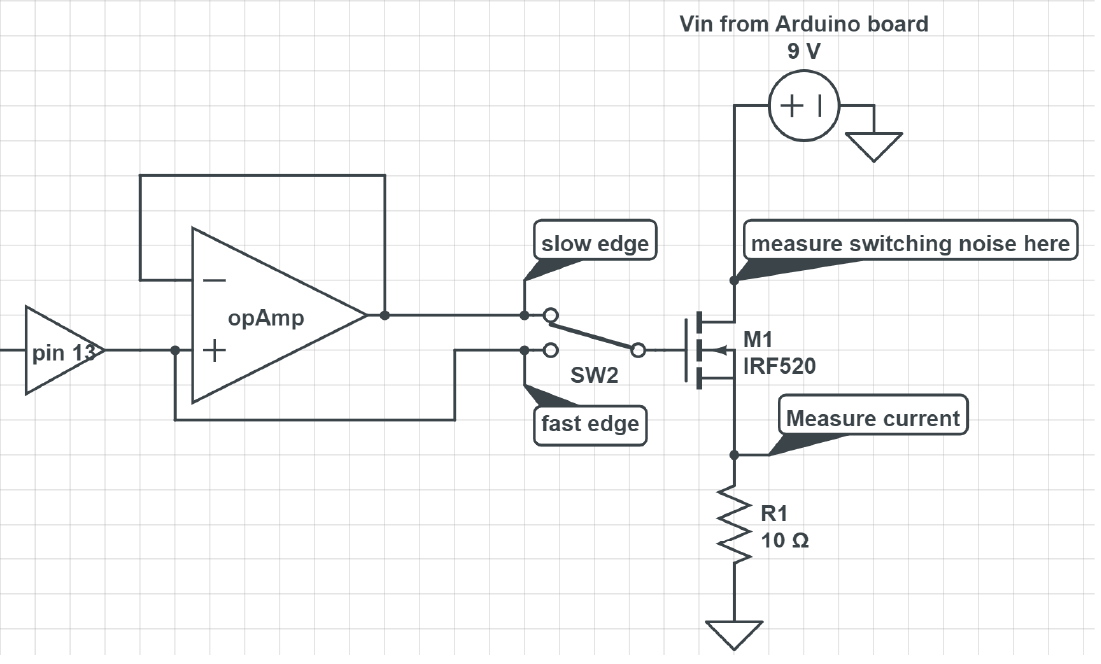
\includegraphics[scale=0.6]{figures/pdn.png}
	\caption{PDN circuit block diagram from book}
	\label{idealbpfilter}
\end{figure}



\pagebreak

\section{Component listing}

\subsection{For Lab Crosstalk and Thevenin R}
	\begin{table}[H]
		\centering

		\begin{tabular}{l c}
			\hline
			\textbf{Component Name}&\textbf{Usecase}\\\hline
			\\
	1 x BNC to BNC Probe&For Signal Generator\\
	1 x 10x Probe&For Oscilloscope \\
	1 x 100 $\ohm$ Resistance&Load Resistance \\
	\hline\hline
		\end{tabular}
		\caption{Lab Crosstalk}
		\label{filterspecs}
	\end{table}

\subsection{For Lab PDNs}
	\begin{table}[H]
		\centering

		\begin{tabular}{l c c c}
			\hline
			\textbf{Component Name}&\textbf{Usecase}&\textbf{Symbol}&\textbf{Value}\\\hline
			&&\\
	1 x Capacitor&Filter Capacitor&C1&10$\mu$F\\
	1 x T272 OPAmp&Slow slew rate opAmp&U1&-\\
	1 x Resistor&Current limiting Resistor&R1&10$\ohm$\\
	1 x N channel MOSFET&For Switching&T1&IRL520\\
	\hline\hline
		\end{tabular}
		\caption{Lab PDN}
		\label{filterspecs}
	\end{table}



\section{Calculations}

Thevenin resistance is the resistance of an entire network reduced to two terminals.


\subsection{Calculating Thevenin Resistance}

    With Independent Sources: Temporarily remove the load resistance (if any) from the circuit. Replace all voltage sources with short circuits and all current sources with open circuits. The resistance seen across the terminals is the Thevenin resistance $R_{th}$.

	\textbf{Isolation of Circuit:} Initially, the load resistance is removed to isolate the circuit. This step is to calculate the inherent resistance of the circuit.


	\begin{table}[!h]
		\centering
	
		\begin{tabular}{c c}
	
			\textbf{Voltage Without Load Resistance}&\textbf{Voltage With Load Resistance}\\
			
			1.01V&0.680V\\\vspace{0.5cm}

		\end{tabular}
		\caption{voltage with and without load resistance}
		\label{voltagewithandwithoutresistance}
	\end{table}

	\textbf{Voltage Measurements:}
		Without Load Resistance: The open-circuit voltage Voc
  is measured across the terminals, which is equivalent to the Thevenin voltage Vth

		With Load Resistance: The circuit voltage Vload
  is measured again after reintroducing the load resistance.

	\begin{flalign*}
	\label{equation_th}
	R_{th} = R_{load}\left(\frac{V_{th} - V_{load}}{V_{load}} \right)
	\end{flalign*}

	\pagebreak

	So first we will measure voltage without load resistance

	\begin{figure}[!h]
		\centering
		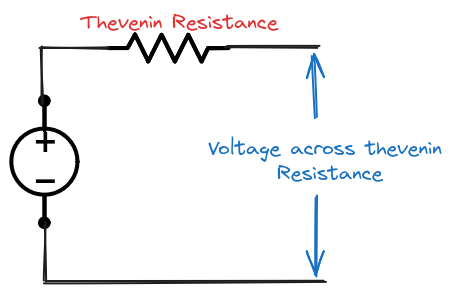
\includegraphics[scale=0.6]{figures/open_th.png}
		\caption{Voltage measurement without load resistance}
		\label{idealbpfilter}
	\end{figure}

	We got around 1.01V of voltage in without load Resistance $R_{load}$.

	Now we will measure Thevenin voltage with load resistance $R_{load}$ of 100$\ohm$.
	
	\begin{figure}[!h]
		\centering
		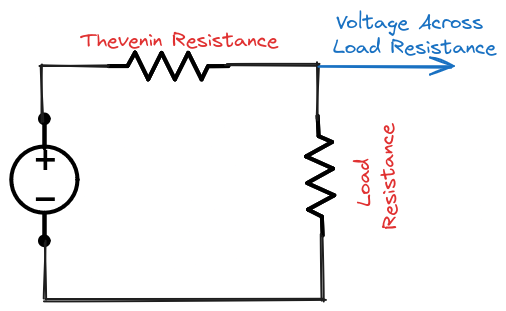
\includegraphics[scale=0.6]{figures/th.png}
		\caption{Voltage drop due to load resistance}
		\label{idealbpfilter}
	\end{figure}

	This time, We got around voltage drop of 0.680V across the load resistance

	and putting values in the equation \ref{equation_th} will give us,

	\begin{flalign*}
		&R_{th} = 100 \left(\frac{1.01 - 0.680}{0.680} \right)&&\\
		&R_{th} = 100 \cdot 0.68529&&\\
		&\boxed{R_{th} = 48.529\ohm}\\
	\end{flalign*}
	

	So conclusion is that the $R_{th}$ of power supply would be around 50$\ohm$.

	\subsection{Cross Talk}


	for the cross talk lab we used signal generator as input to oscilloscope and we shorted the output of waveform generator and oscilloscopes and we put the loop of the probes to signal generator and due to switching of the voltage and current, new current (noise) was generated in the other loop (L) and this noise due to loop inductance is called crosstalk

	\textbf{dI/dT Impact:} The rate of change of current (dI/dT) plays role in the intensity of the crosstalk. Higher dI/dT values, typically found in short rise time current transients, result in more pronounced power rail noise.In our case large loop inductance is causing crosstalk currents to induce in oscilloscope loop

	\textbf{Circuit Behavior:} This behavior aligns with the principle that circuits requiring power rapidly can induce significant voltage fluctuations and noise on the power rail.

	\begin{figure}[!h]
		\centering
		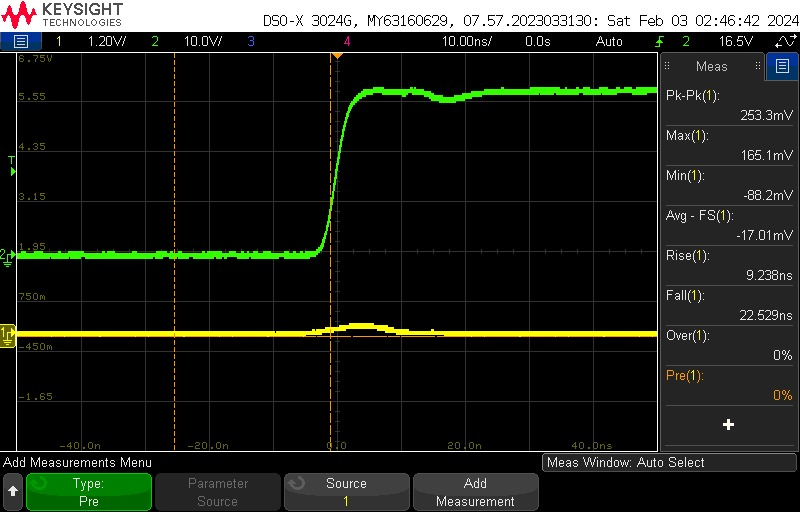
\includegraphics[scale=0.6]{figures/noise_crosstalk.jpeg}
		\caption{Noise/Crosstalk in Oscilloscope Probe}
	\end{figure}

	\begin{figure}[!h]
		\centering
		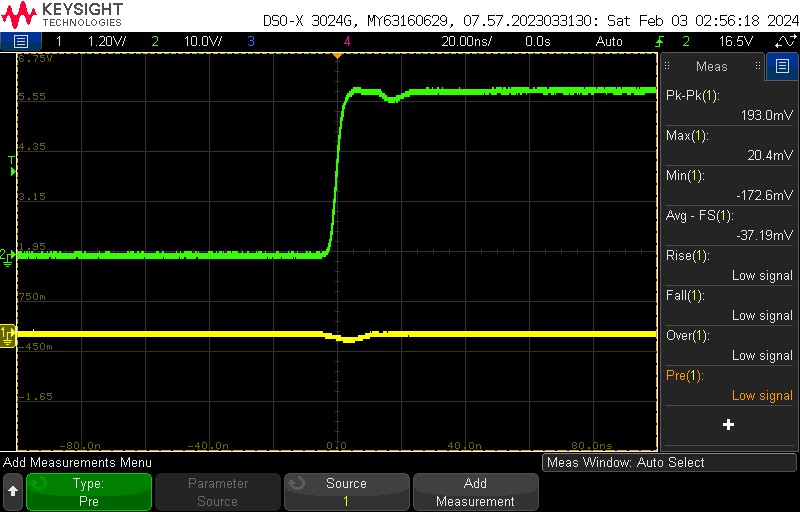
\includegraphics[scale=0.6]{figures/noise_crosstalk2.jpeg}
		\caption{Noise/Crosstalk in Oscilloscope Probe - 2}
	\end{figure}

	\subsection{Calculating Power rail noise due to switching}



		The experiments focused on understanding the behavior of a slammer circuit on a solder less breadboard with focus switching noise, power consumption, and the effects of different rise times and decoupling capacitors.

	
		Rise and Fall time for Arduino digital output is mentioned below
		
		\begin{table}[H]
			\centering
		
			\begin{tabular}{l c c}
		
				&\textbf{Rise Time}&\textbf{Fall Time}\\\hline
				&&\\
				\textbf{Arduino}&13ns&25ns\\
				\textbf{OPAmp}&1.4$\mu$s&1.4$\mu$s\\
		
			\end{tabular}
			\caption{Rise-time and Fall-time}
			\label{tab_rise_fall}
		\end{table}
			
		And according to data-sheet opAmp's slew rate was around 1.5 $\mu$sec/V , From the observation we can see that the rising and falling edge compliance with the data-sheet

		Current going through Resistor was measured with the series Ammeter, here is the results of Ammeter


		\begin{figure}[H]
			\centering
			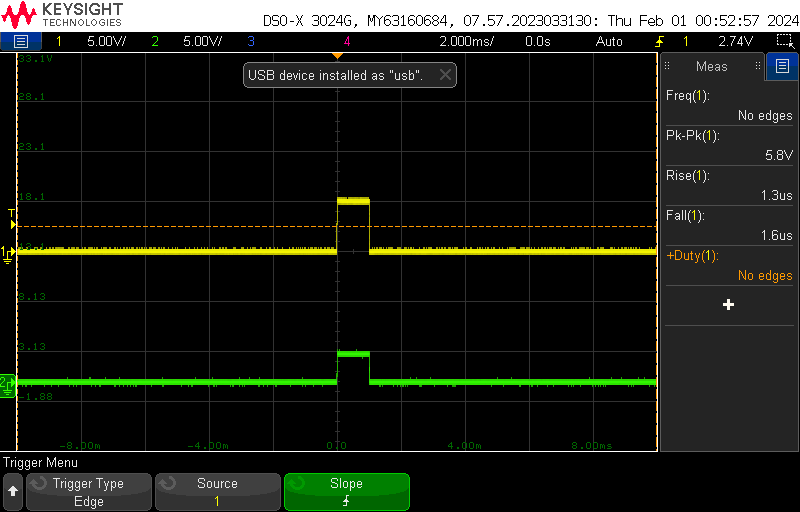
\includegraphics[scale=0.6]{figures/opo_fetin1.png}
			\caption{OpAmp Output and MOSFET Gate}
		\end{figure}

	
		Two Driver Signals to Transistor’s Base: The setup included two signals to drive the MOSFET: the raw input from the Arduino and the buffered output from the opAmp follower. The rise and fall times of these signals were measured, and their impact on the circuit's performance was observed.
	

	
		\subsection{Initial Measurement with Slow Rise Time Signal:}
		The slow rise time signal from the opAmp output was first connected to the MOSFET gate. The voltage at the opAmp output was measured, showing a long rise time.

		here is the noise on the power rail due to slower rising edge  
		\begin{figure}[H]
			\centering
			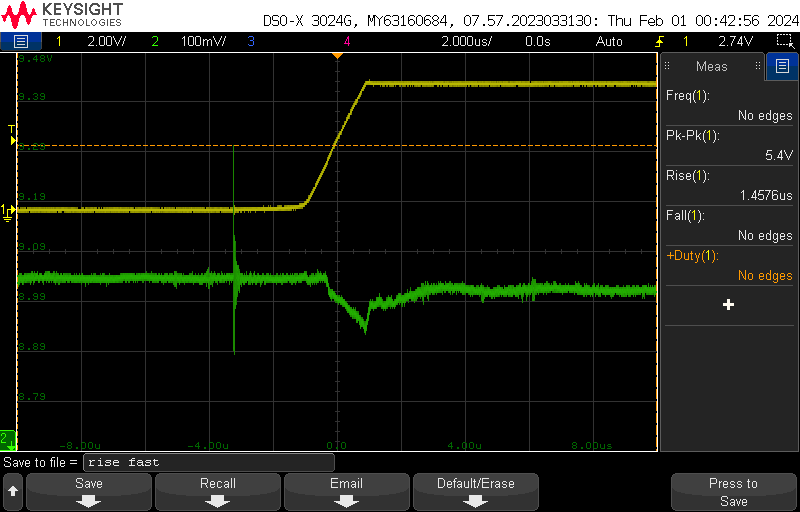
\includegraphics[scale=0.6]{figures/rise_slow.png}
			\caption{slower rising edge}
		\end{figure}
		
		here is the noise on the power rail due to slower falling edge 
		\begin{figure}[H]
			\centering
			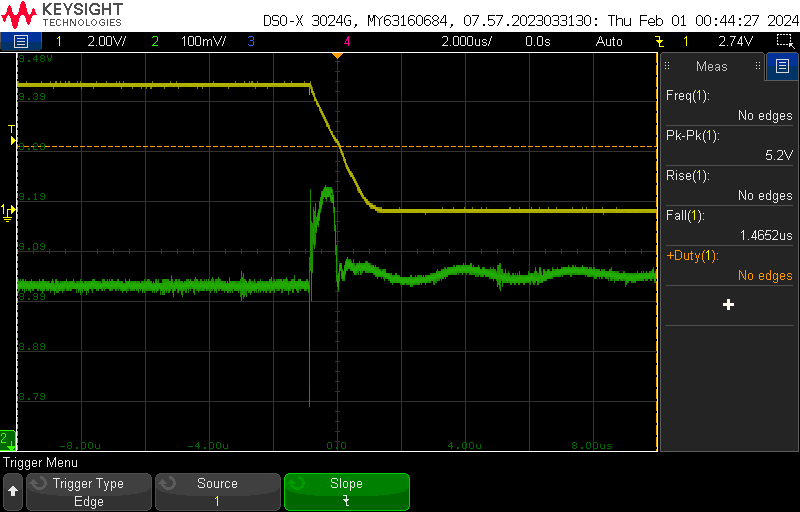
\includegraphics[scale=0.6]{figures/fall_slow.png}
			\caption{slower falling edge }
		\end{figure}

		Noise due to slow rising and falling edge does not cause much of fluctuations on power rail of the bread board and reason is dI/dt is not changing abruptly and causing high mutual impedance in the power rail.

		\subsection{Measurement with Fast Rise Time Signal:}
		The fast rise time signal from the Arduino output was directly connected to the MOSFET gate. The voltage at the Arduino output was measured, showing a fast rise time.\\

		Noise on the power rail due to fast rising edge  
		\begin{figure}[H]
			\centering
			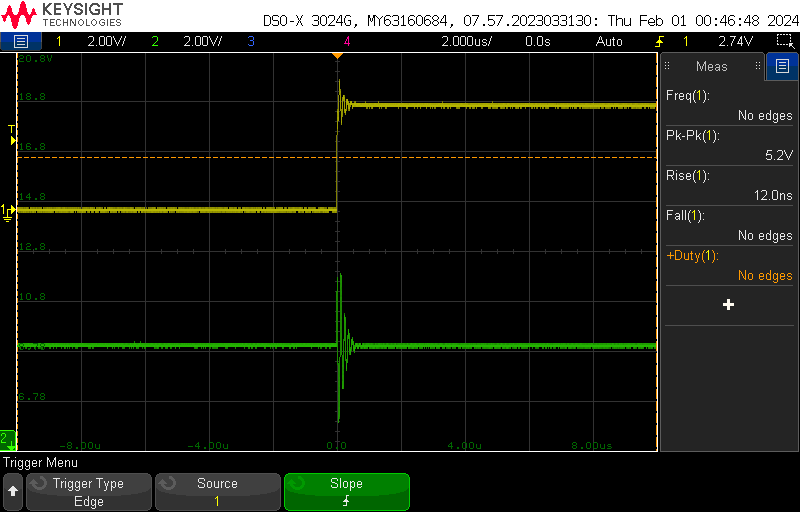
\includegraphics[scale=0.6]{figures/fast_rise.png}
			\caption{fast rising edge}
		\end{figure}

	
		here is the noise on the power rail due to fast falling edge 
		\begin{figure}[H]
			\centering
			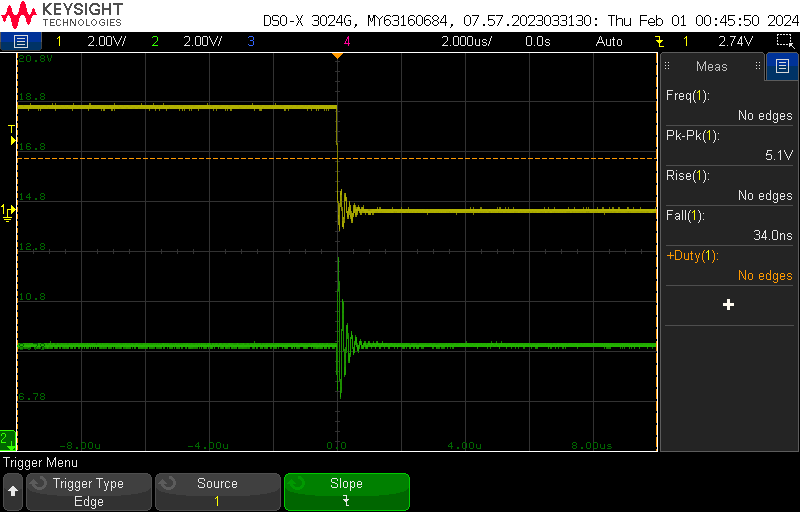
\includegraphics[scale=0.6]{figures/fast_fall.png}
			\caption{fast falling edge }
		\end{figure}

		Here we can see the noise is very high due to fast switching and this was measured around 300mV peak to peak voltage noise on power rail
	

		\subsection{Adding Decoupling Capacitors}


		here is the noise on the power rail due to slower rising edge with 10$\mu$F capacitor added in the power rail as close as to opAmp.

		\begin{figure}[H]
			\centering
			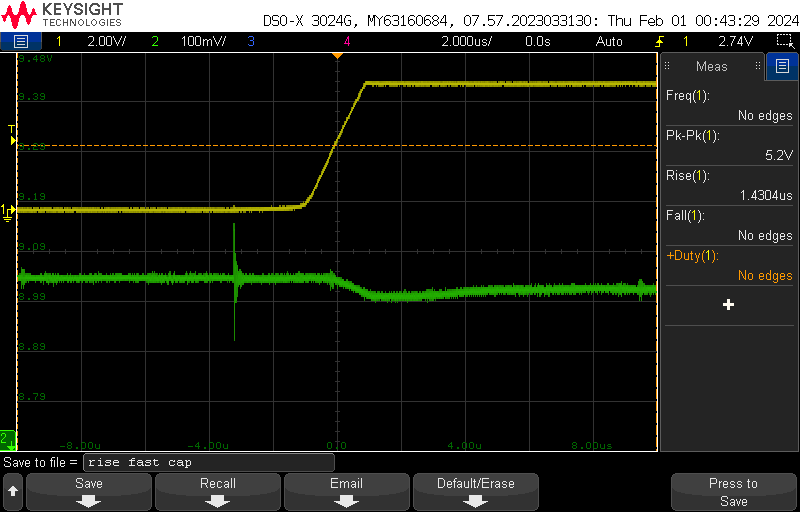
\includegraphics[scale=0.6]{figures/rise_slow_cap.png}
			\caption{slower rising edge with capacitor added}
		\end{figure}

		here is the noise on the power rail due to slower falling edge with 10$\mu$F capacitor added in the power rail as close as to opAmp.

		\begin{figure}[H]
			\centering
			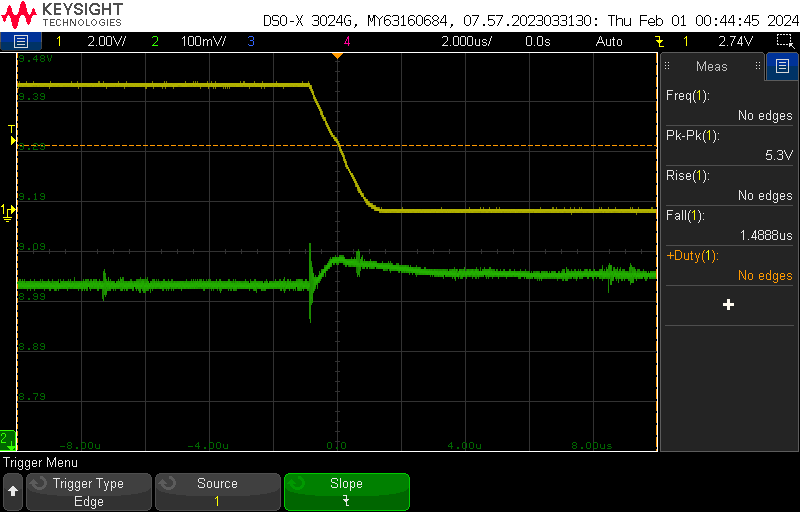
\includegraphics[scale=0.6]{figures/fall_slow_cap.png}
			\caption{slower falling edge with capacitor added}
		\end{figure}

		\pagebreak
		here is the noise on the power rail due to \textbf{fast rising edge} with 10$\mu$F capacitor added in the power rail as close as to opAmp.

		\begin{figure}[H]
			\centering
			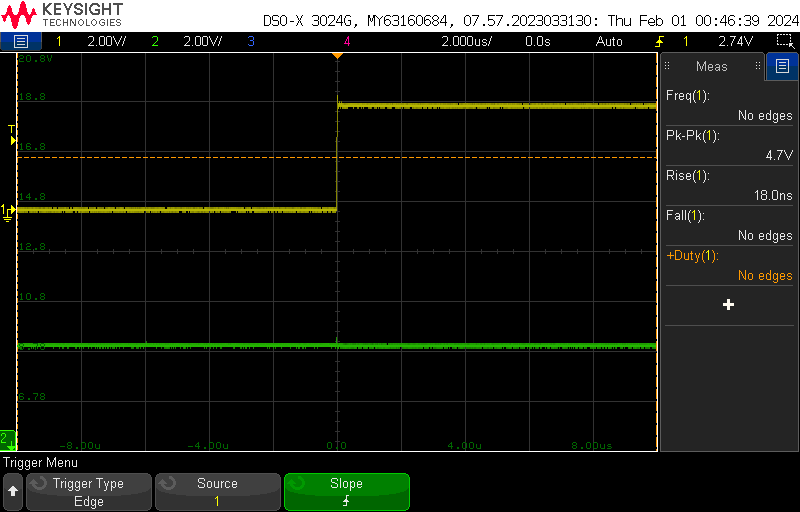
\includegraphics[scale=0.6]{figures/fast_rise_cap.png}
			\caption{fast rising edge with capacitor added}
		\end{figure}

		here is the noise on the power rail due to \textbf{fast falling edge} with 10$\mu$F capacitor added in the power rail as close as to opAmp.

		\begin{figure}[H]
			\centering
			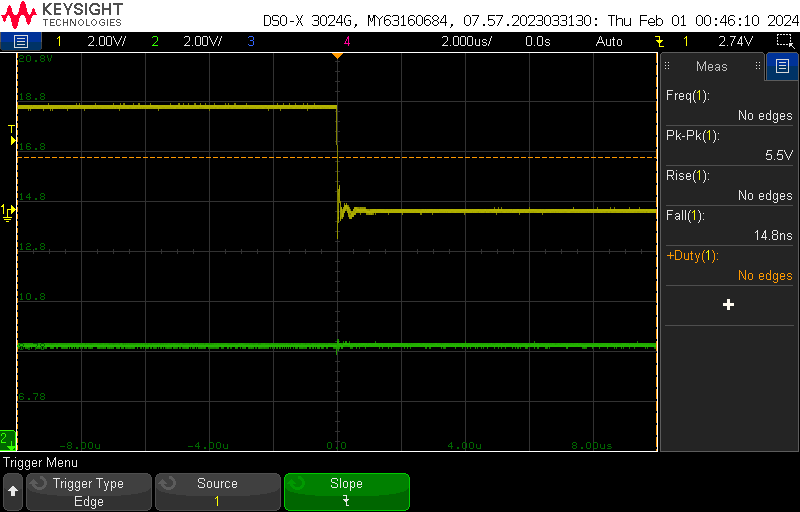
\includegraphics[scale=0.6]{figures/fast_fall_cap.png}
			\caption{fast falling edge with capacitor added}
		\end{figure}
		
		\subsection{Observation of Switching Noise Characteristics:}

		
This observed behavior in the circuit is attributed to the power demand dynamics. When the circuit requires power, particularly during high consumption periods, there is a corresponding drop in voltage along the voltage rail. This voltage drop, in turn, is the primary cause of the observed noise on the power rail. The extent of this voltage fluctuation and the resultant noise is directly related to the current demand of the circuit at any given moment. Such fluctuations are particularly pronounced during instances of sudden or high current draw, which are common in circuits with rapidly switching components or those undergoing transient states. This phenomenon underscores the importance of stable power supply design and the implementation of noise mitigation strategies, such as decoupling capacitors, to maintain consistent voltage levels and minimize noise interference in the power rail.






		

		\subsection{Estimating Decoupling Capacitor Size}
		During the time of the rising or falling edge, \( dt \), when there will be inductive switching noise, we want all of the current \( I \) to come from the capacitor, so none of it has to flow through the rest of the inductance of the power rail. However, this current only needs to flow during the rising or falling edge. If we want to limit the voltage drop, during the \( dt \) time, to 0.4 V, for example, the capacitance \( C \) we need is calculated as follows:
	(From the lab manual)
		\begin{equation}
		C = \frac{I \times dt}{\Delta V} = \frac{0.4 \times 1\, \mu\text{sec}}{0.4\, V} = 1\, \mu F
		\end{equation}

		\subsection{Decoupling Capacitor Location}
		
		A notable observation was the reduction in noise levels when a 10 µF capacitor was placed close to the opAmp, that causes charge storage in smoothing out voltage fluctuations caused by rapid current changes.




\section{Conclusion}

The lab demonstrated the characteristics of noise how it is generated how it affects the circuit and how it can be reduced, by removing loop inductance adding decoupling capacitor, also keeping in mind the rise time and fall time of the elements while designing the circuit

\begin{enumerate}
	\item \textbf{Effects of Rise and Fall Times:}

	The speed at which signals in a circuit change, called rise and fall times, can affect how much noise is seen in the power supply. Faster changes tend to create more noise.
	\item \textbf{Role of Decoupling Capacitors:}
	
	We learned that capacitors can help reduce noise in a circuit. Their size and where they are placed in the circuit can make a big difference in how effective they are.
	\item\textbf{Analyzing Noise:}
	
	By looking at different types of noise on the power rail, we understood more about how circuits can affect power supplies. We saw that noise can change depending on many factors, like how fast a signal changes or where components are locate

	\item \textbf{Understanding Crosstalk:}

	The lab provided a clear demonstration of crosstalk, an unwanted phenomenon where a signal in one circuit or channel creates an undesired effect in another.
\end{enumerate}


Breadboard Implementation:

\begin{figure}[H]
	\centering
	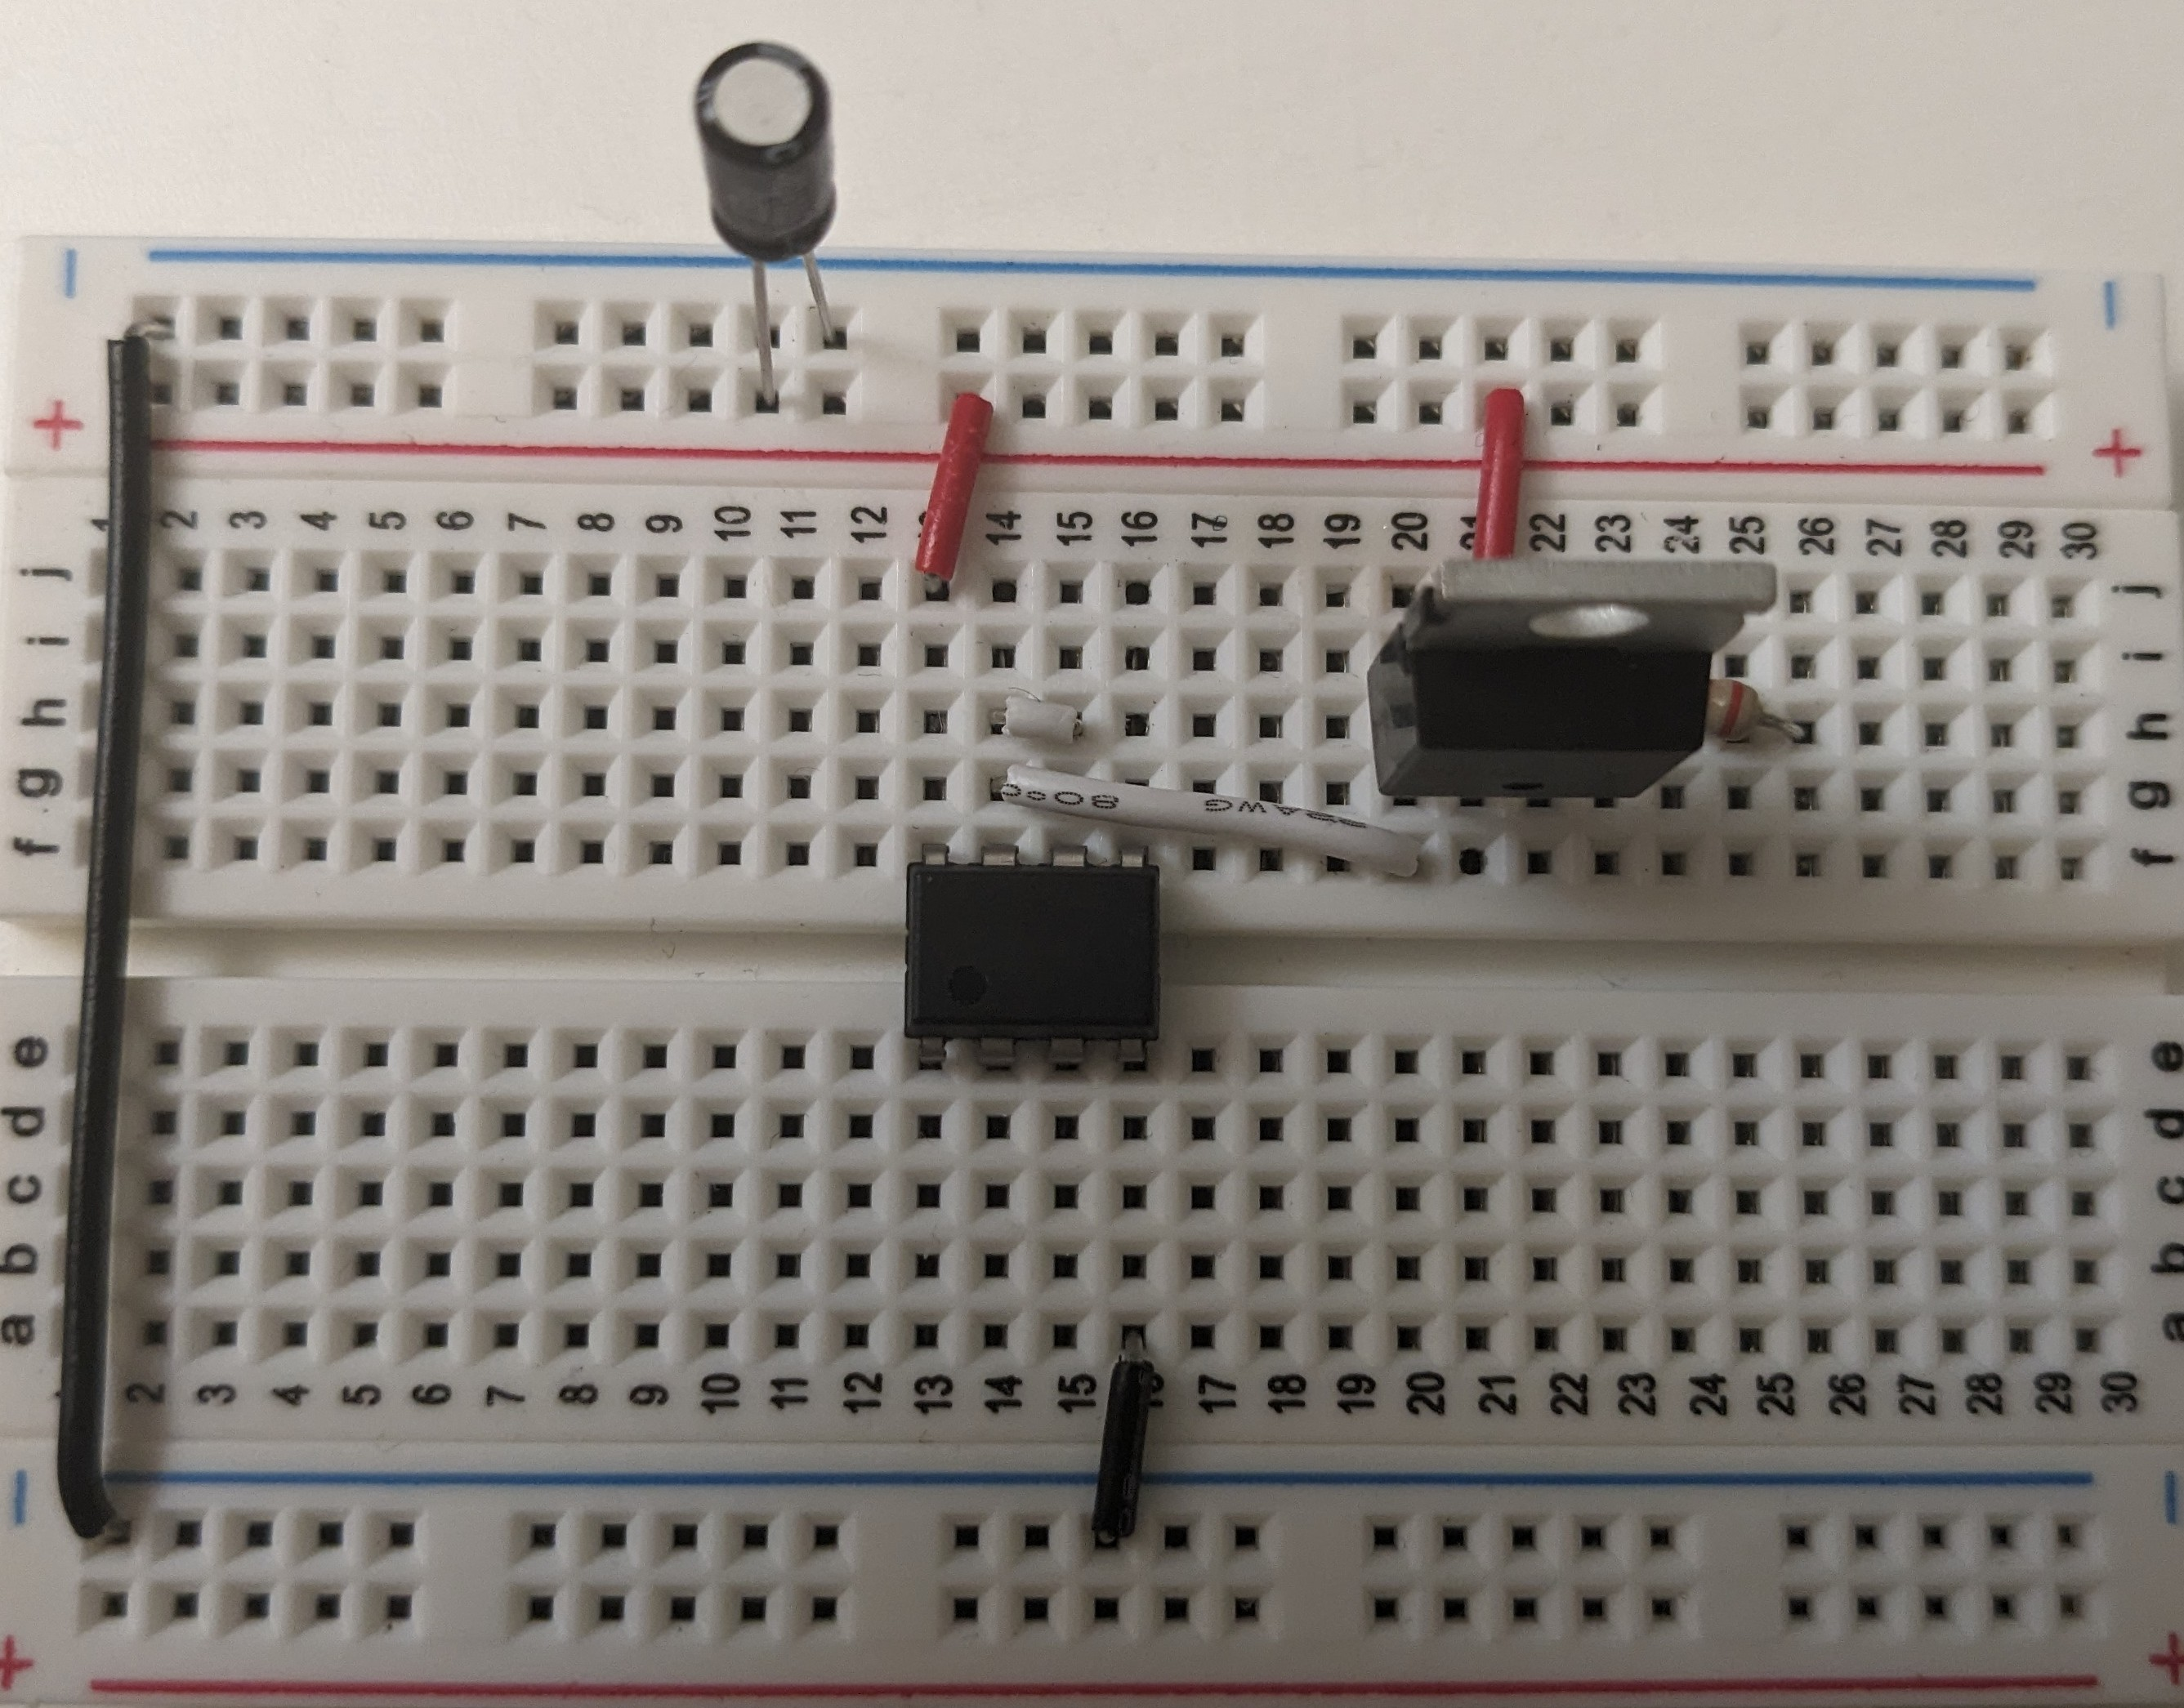
\includegraphics[scale=0.12]{figures/breadboard.jpg}
	\caption{Breadboard Implementation}
	\label{breadboard}
\end{figure}

\hrule






%---------------------------------------------------------------------------
\end{document}
-
